\documentclass[10pt]{beamer}\usepackage[]{graphicx}\usepackage[]{color}
% maxwidth is the original width if it is less than linewidth
% otherwise use linewidth (to make sure the graphics do not exceed the margin)
\makeatletter
\def\maxwidth{ %
  \ifdim\Gin@nat@width>\linewidth
    \linewidth
  \else
    \Gin@nat@width
  \fi
}
\makeatother

\definecolor{fgcolor}{rgb}{0.345, 0.345, 0.345}
\newcommand{\hlnum}[1]{\textcolor[rgb]{0.686,0.059,0.569}{#1}}%
\newcommand{\hlstr}[1]{\textcolor[rgb]{0.192,0.494,0.8}{#1}}%
\newcommand{\hlcom}[1]{\textcolor[rgb]{0.678,0.584,0.686}{\textit{#1}}}%
\newcommand{\hlopt}[1]{\textcolor[rgb]{0,0,0}{#1}}%
\newcommand{\hlstd}[1]{\textcolor[rgb]{0.345,0.345,0.345}{#1}}%
\newcommand{\hlkwa}[1]{\textcolor[rgb]{0.161,0.373,0.58}{\textbf{#1}}}%
\newcommand{\hlkwb}[1]{\textcolor[rgb]{0.69,0.353,0.396}{#1}}%
\newcommand{\hlkwc}[1]{\textcolor[rgb]{0.333,0.667,0.333}{#1}}%
\newcommand{\hlkwd}[1]{\textcolor[rgb]{0.737,0.353,0.396}{\textbf{#1}}}%
\let\hlipl\hlkwb

\usepackage{framed}
\makeatletter
\newenvironment{kframe}{%
 \def\at@end@of@kframe{}%
 \ifinner\ifhmode%
  \def\at@end@of@kframe{\end{minipage}}%
  \begin{minipage}{\columnwidth}%
 \fi\fi%
 \def\FrameCommand##1{\hskip\@totalleftmargin \hskip-\fboxsep
 \colorbox{shadecolor}{##1}\hskip-\fboxsep
     % There is no \\@totalrightmargin, so:
     \hskip-\linewidth \hskip-\@totalleftmargin \hskip\columnwidth}%
 \MakeFramed {\advance\hsize-\width
   \@totalleftmargin\z@ \linewidth\hsize
   \@setminipage}}%
 {\par\unskip\endMakeFramed%
 \at@end@of@kframe}
\makeatother

\definecolor{shadecolor}{rgb}{.97, .97, .97}
\definecolor{messagecolor}{rgb}{0, 0, 0}
\definecolor{warningcolor}{rgb}{1, 0, 1}
\definecolor{errorcolor}{rgb}{1, 0, 0}
\newenvironment{knitrout}{}{} % an empty environment to be redefined in TeX

\usepackage{alltt}

\beamertemplatenavigationsymbolsempty

\usepackage{colortbl}
\usepackage{tikz}
\usetikzlibrary{calc}
\usetikzlibrary{intersections}
\usetikzlibrary{datavisualization}
\usetikzlibrary{datavisualization.formats.functions}

\newcommand\lo{\ensuremath{\boldsymbol{-}}}
\newcommand\hi{\ensuremath{\boldsymbol{+}}}
\newcommand\sst{SS_\mathrm{total}}
\newcommand\ssx{SS_\mathrm{explained}}
\newcommand\ssr{SS_\mathrm{residual}}

\newcommand\y{\mathbf{y}}
\newcommand\mean{\mathrm{mean}}
\newcommand\pred{\mathrm{predicted}}

\title{Factorial Designs}
\author{BIOE 498/598 PJ}
\date{Spring 2021}
\IfFileExists{upquote.sty}{\usepackage{upquote}}{}
\begin{document}
%\SweaveOpts{concordance=TRUE}

\frame{\titlepage}


\begin{frame}{The sum of squares}

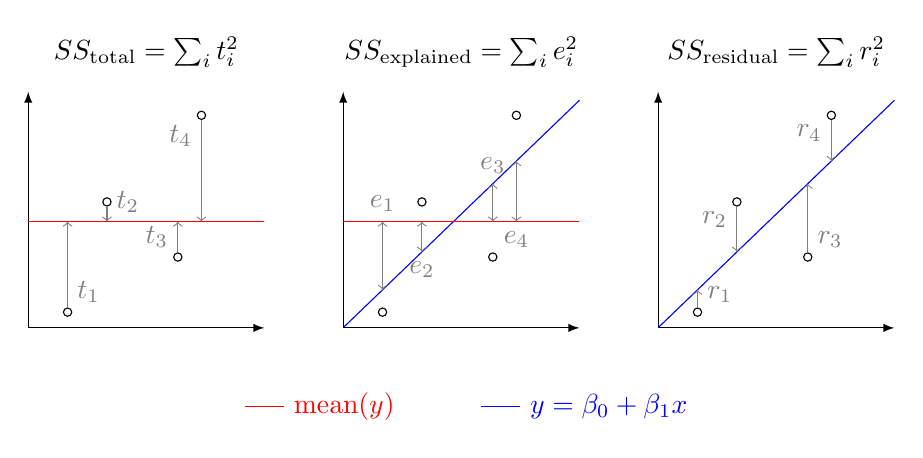
\begin{tikzpicture}
\begin{scope}
	\draw [->,>=latex] (0,0) -- (3,0);
	\draw [->,>=latex] (0,0) -- (0,3);
	
	\draw [name path=mean,domain=0:3,red] plot (\x, {1.35});
	
	\foreach \pt/\i in {(0.5,0.2)/1, (1.9,0.9)/3, (2.2,2.7)/4, (1.0,1.6)/2} {
		\node [draw,circle,minimum size=3pt,inner sep=0pt] (nd\i) at \pt {};
		\path [name path=path\i] let \p1 = \pt in (\x1,0) -- (\x1,3);
		\draw [name intersections={of={path\i} and mean},->,gray] (nd\i) -- (intersection-1);
	}
	\node [above right,gray] at (nd1) {$t_1$};
	\node [right,gray] at (nd2) {$t_2$};
	\node [above left,gray] at (nd3) {$t_3$};
	\node [below left,gray] at (nd4) {$t_4$};
	\node at (1.5,3.5) {$SS_\mathrm{total} = \sum_i t_i^2$};
\end{scope}

\begin{scope}[shift={(4cm,0)}]
	\draw [->,>=latex] (0,0) -- (3,0);
	\draw [->,>=latex] (0,0) -- (0,3);
	
	\draw [name path=model,domain=0:3,blue] plot (\x, {0.0027 + 0.9624*\x});
	\draw [name path=mean,domain=0:3,red] plot (\x, {1.35});
	
	\foreach \pt/\i in {(0.5,0.2)/1, (1.0,1.6)/2, (1.9,0.9)/3, (2.2,2.7)/4} {
		\node [draw, circle, minimum size=3pt, inner sep=0pt] (nd\i) at \pt {};
		\path [name path=path\i] let \p1 = \pt in (\x1,0) -- (\x1,3);
		\draw [
			name intersections={of=model and path\i, name={mdint\i}},
			name intersections={of=mean and path\i, name={mnint\i}},
			gray,<->
		] (mdint\i-1) -- (mnint\i-1);
	}
	
	\node [above,gray] at (mnint1-1) {$e_1$};
	\node [below,gray] at (mdint2-1) {$e_2$};
	\node [above,gray] at (mdint3-1) {$e_3$};
	\node [below,gray] at (mnint4-1) {$e_4$};
	
	\node at (1.5,3.5) {$SS_\mathrm{explained} = \sum_i e_i^2$};
\end{scope}

\begin{scope}[shift={(8cm,0)}]
	\draw [->,>=latex] (0,0) -- (3,0);
	\draw [->,>=latex] (0,0) -- (0,3);
	
	\draw [name path=model,domain=0:3,blue] plot (\x, {0.0027 + 0.9624*\x});
	
	\foreach \pt/\i in {(0.5,0.2)/1, (1.9,0.9)/3, (2.2,2.7)/4, (1.0,1.6)/2} {
		\node [draw,circle,minimum size=3pt,inner sep=0pt] (nd\i) at \pt {};
		\path [name path=path\i] let \p1 = \pt in (\x1,0) -- (\x1,3);
		\draw [name intersections={of={path\i} and model},->,gray] (nd\i) -- (intersection-1);
	}
	\node [above right,gray] at (nd1) {$r_1$};
	\node [below left,gray] at (nd2) {$r_2$};
	\node [above right,gray] at (nd3) {$r_3$};
	\node [below left,gray] at (nd4) {$r_4$};
	\node at (1.5,3.5) {$SS_\mathrm{residual} = \sum_i r_i^2$};
\end{scope}

\draw [red] (2.75,-1) -- ++(0.5,0) node[right,red] {$\mathrm{mean}(y)$} ++(2,0);
\draw [blue] (5.75,-1) -- ++(0.5,0) node[right,blue] {$y = \beta_0 + \beta_1x$};
\end{tikzpicture}

\pause
\[ \sst = \ssx + \ssr \]

\end{frame}

\begin{frame}{The sum of squares}

Our analysis is based on the \emph{sum of squares}, or SS. In particular, the total SS is the combination of the SS explained by our model and the SS that is residual (or unexplained).

\[ \sst = \ssx + \ssr \]

\pause
How do we calculate each one for a model $\y = \mathbf{X}\mathbf{\beta}$?

\pause
\[ \sst = \sum_i (y_i - \mean(\y))^2 \]
\pause
\[ \ssr = \sum_i (y_i - \pred(y_i))^2 \]
\pause
\[ \ssx = \sst - \ssr \]

\end{frame}

\begin{frame}[fragile]{Does our model do anything?}

Let's analyze the data from the stuffed monkey throwing experiment.
\footnotesize
\begin{knitrout}
\definecolor{shadecolor}{rgb}{0.969, 0.969, 0.969}\color{fgcolor}\begin{kframe}
\begin{verbatim}
## 
## Call:
## lm(formula = distance ~ hand + hat + boots)
## 
## Residuals:
##      1      2      3      4      5      6      7      8 
## -0.375 -1.125  0.625  0.875  1.125  0.375 -1.375 -0.125 
## 
## Coefficients:
##             Estimate Std. Error t value Pr(>|t|)   
## (Intercept)    5.375      0.857   6.272   0.0033 **
## handright      2.250      0.857   2.626   0.0585 . 
## hatyes        -1.500      0.857  -1.750   0.1549   
## bootsyes       1.000      0.857   1.167   0.3081   
## ---
## Signif. codes:  0 '***' 0.001 '**' 0.01 '*' 0.05 '.' 0.1 ' ' 1
## 
## Residual standard error: 1.212 on 4 degrees of freedom
## Multiple R-squared:  0.7389,	Adjusted R-squared:  0.5431 
## F-statistic: 3.773 on 3 and 4 DF,  p-value: 0.1161
\end{verbatim}
\end{kframe}
\end{knitrout}

\end{frame}

\begin{frame}[fragile]{For our throwing data}

\begin{knitrout}
\definecolor{shadecolor}{rgb}{0.969, 0.969, 0.969}\color{fgcolor}\begin{kframe}
\begin{alltt}
\hlstd{ss} \hlkwb{<-} \hlkwa{function}\hlstd{(}\hlkwc{x}\hlstd{)} \hlkwd{sum}\hlstd{(x}\hlopt{^}\hlnum{2}\hlstd{)}
\hlstd{sst} \hlkwb{<-} \hlkwd{ss}\hlstd{(distance} \hlopt{-} \hlkwd{mean}\hlstd{(distance))}
\hlstd{ssr} \hlkwb{<-} \hlkwd{ss}\hlstd{(}\hlkwd{residuals}\hlstd{(model))}
\hlstd{ssx} \hlkwb{<-} \hlstd{sst} \hlopt{-} \hlstd{ssr}
\hlkwd{c}\hlstd{(sst, ssr, ssx)}
\end{alltt}
\begin{verbatim}
## [1] 22.500  5.875 16.625
\end{verbatim}
\end{kframe}
\end{knitrout}

\end{frame}

\begin{frame}[fragile]{Degrees of freedom}

The amount of variation we expect to see depends on the number of independent parameters in the model. These are the \emph{degrees of freedom}, and we need to normalize the SS by them.

For analyzing variation, the number of parameters does not include the intercept.

\begin{itemize}
  \item For $\sst$, DF = (\# data points) - 1
  \item For $\ssx$, DF = \# of parameters
  \item For $\ssr$, DF = (\# data points) - (\# parameters) - 1
\end{itemize}

\end{frame}

\begin{frame}{The $F$-statistic}

The value of our model is explained by the ratio between the explained variance and the residual (unexplained) variance \emph{after adjusting for the DF}.

\[ F = \frac{\ssx / \mathrm{DF}(\ssx)}{\ssr / \mathrm{DF}(\ssr)} \]

\pause
For our throwing example

\[ F = \frac{16.625 /3}{5.875 / (8-3-1)} = 3.773 \]

\pause
\textbf{How big should the $F$-statistic be?} The $F$-statistic follows the $F$-distribution. We can use this distribution to convert the $F$-statistic into a $p$-value.

\end{frame}

\begin{frame}[fragile]

\begin{knitrout}
\definecolor{shadecolor}{rgb}{0.969, 0.969, 0.969}\color{fgcolor}\begin{kframe}
\begin{alltt}
\hlkwd{summary}\hlstd{(model)}
\end{alltt}
\begin{verbatim}
## 
## Call:
## lm(formula = distance ~ hand + hat + boots)
## 
## Residuals:
##      1      2      3      4      5      6      7      8 
## -0.375 -1.125  0.625  0.875  1.125  0.375 -1.375 -0.125 
## 
## Coefficients:
##             Estimate Std. Error t value Pr(>|t|)   
## (Intercept)    5.375      0.857   6.272   0.0033 **
## handright      2.250      0.857   2.626   0.0585 . 
## hatyes        -1.500      0.857  -1.750   0.1549   
## bootsyes       1.000      0.857   1.167   0.3081   
## ---
## Signif. codes:  0 '***' 0.001 '**' 0.01 '*' 0.05 '.' 0.1 ' ' 1
## 
## Residual standard error: 1.212 on 4 degrees of freedom
## Multiple R-squared:  0.7389,	Adjusted R-squared:  0.5431 
## F-statistic: 3.773 on 3 and 4 DF,  p-value: 0.1161
\end{verbatim}
\end{kframe}
\end{knitrout}

\end{frame}

\begin{frame}{Testing single factors}

We previously compared the entire model against the residuals to see if the model added value. We can apply the same procedure to a single variable.

This is called the \emph{analysis of variance}, or ANOVA.

\end{frame}

\begin{frame}[fragile]{ANOVA on handedness}

Let's find the explained variance for a model with only handedness:
\small
\begin{knitrout}
\definecolor{shadecolor}{rgb}{0.969, 0.969, 0.969}\color{fgcolor}\begin{kframe}
\begin{alltt}
\hlstd{model_hand} \hlkwb{<-} \hlkwd{lm}\hlstd{(distance} \hlopt{~} \hlstd{hand)}
\hlstd{sst} \hlopt{-} \hlkwd{ss}\hlstd{(}\hlkwd{residuals}\hlstd{(model_hand))}
\end{alltt}
\begin{verbatim}
## [1] 10.125
\end{verbatim}
\end{kframe}
\end{knitrout}
\normalsize
Now let's compare this to the residuals of the entire model:

\pause
\[ F = \frac{10.125 /1}{5.875 / (8-3-1)} = 6.894 \]

\end{frame}

\begin{frame}[fragile]{ANOVA on a linear model}

We can repeat this procedure for every variable, or we can use R's built-in ANOVA command.
\begin{knitrout}
\definecolor{shadecolor}{rgb}{0.969, 0.969, 0.969}\color{fgcolor}\begin{kframe}
\begin{alltt}
\hlkwd{anova}\hlstd{(model)}
\end{alltt}
\begin{verbatim}
## Analysis of Variance Table
## 
## Response: distance
##           Df Sum Sq Mean Sq F value  Pr(>F)  
## hand       1 10.125 10.1250  6.8936 0.05846 .
## hat        1  4.500  4.5000  3.0638 0.15495  
## boots      1  2.000  2.0000  1.3617 0.30807  
## Residuals  4  5.875  1.4688                  
## ---
## Signif. codes:  0 '***' 0.001 '**' 0.01 '*' 0.05 '.' 0.1 ' ' 1
\end{verbatim}
\end{kframe}
\end{knitrout}

\end{frame}

\begin{frame}{Conclusions}

\begin{itemize}
  \item $p$-values on effect sizes tell us if the effect size in nonzero.
  \item A significant effect size does not mean the effect matters.
  \item ANOVA can tell us which variables explain a significant fraction of the variance in our data.
  \item Significance is realtive to the unexplained variance in the model.
\end{itemize}

\end{frame}

\end{document}
